\documentclass[a4paper,11pt]{article}
\pdfoutput=1 % if your are submitting a pdflatex (i.e. if you have
             % images in pdf, png or jpg format)

\usepackage{jinstpub} % for details on the use of the package, please
\usepackage{titlesec}                     % see the JINST-author-manual
\usepackage{parskip}
\usepackage{float}
\titlespacing{\section}{0pt}{\parskip}{2pt}
%\titlespacing{\subsection}{0pt}{\parskip}{-\parskip}
\titlespacing{\subsubsection}{0pt}{\parskip}{-\parskip}

\title{\boldmath Detector Control System for CMS RPC at GIF++}


%% %simple case: 2 authors, same institution
% \author{Muhammad Gul }
% \affiliation{Ghent University,\\Belgium}

% more complex case: 4 authors, 3 institutions, 2 footnotes
\author[a,1]{M. Gul,\note{Corresponding author.}} 
\author[a]{M. Tytgat, N. Zaganidis, A. A. O. Rios, A. Fagot, S. Crucy, A. Cimmino}\affiliation[a]{Ghent University, Department of Physics and Astronomy, Proeftuinstraat 86, 9000 Gent, Belgium.}
\author[b]{Y. Assran, A. Radi, S. Ali, A. Sayed}\affiliation[b]{Egyptian Network for High Energy Physics, Academy of Scientific Research and Technology, 101 Kasr El-Einy St. Cairo Egypt.}
\author[c]{G. Singh}\affiliation[c]{Chulalongkorn University, Department of Physics, Faculty of Science, Payathai Road, Phatumwan, Bangkok, THAILAND - 10330.}
\author[d]{M. Abbrescia, G. Iaselli, M. Maggi, G. Pugliese, P. Verwilligen}\affiliation[d]{INFN, Sezione di Bari, Via Orabona 4, IT-70126 Bari, Italy.}
\author[e]{W. van Doninck}\affiliation[e]{Vrije Universiteit Brussel, Boulevard de la Plaine 2, 1050 Ixelles, Belgium.}
\author[f]{S. Colafranceschi, A. Sharma}\affiliation[f]{Physics Department CERN, CH-1211 Geneva 23, Switzerland.}
\author[g]{L. Benussi, S. Bianco, D. Piccolo, F. primavera}\affiliation[g]{INFN, Laboratori Nazionali di Frascati (LNF), Via Enrico Fermi 40, IT-00044 Frascati, Italy.}
\author[h]{V. Bhatnagar, J. Singh, R. kumar, A. Metha}\affiliation[h]{Department of Physics, Panjab University, Chandigarh Mandir 160 014, India.}
\author[i]{A. Ahmad, M. Ahmad, Q. Hassan, H. R. Hoorani, W. A. Khan, T. Khurshid}\affiliation[i]{National Centre for Physics, Quaid-i-Azam University, Islamabad, Pakistan.}
\author[j]{S. Choi, B. S. Hong, M. Jo, H. Kim, K. Lee, K. S. Lee, S. K. Park, J. W. Kang, M. Kang}\affiliation[j]{Korea University, Department of Physics, Seoul Cheongryangri 143-701, Republic of Korea}
\author[k]{D.H. Kim}\affiliation[k]{Kyungpook National University, Daegu, Korea.}
\author[l]{S.K. Nam}\affiliation[l]{Kangwon National University, Chunchon, Korea.}
\author[m]{G. Grenier, M. Goutzvitz, F. Lagarde, I.B. Laktineh}\affiliation[m]{Universit  ́e de Lyon, Universit  ́e Claude Bernard Lyon 1,  CNRS-IN2P3, Institut de Physique Nucl  ́eaire de Lyon, Villeurbanne, France.}
\author[n]{U. E. Cecilia, I. Pedraza, C. B. Severiano}\affiliation[n]{Benemerita Universidad Autonoma de Puebla, Puebla, Mexico.}
\author[o]{S. Carrillo Moreno, F. Vazquez Valencia}\affiliation[o]{Universidad Iberoamericana, Mexico City, Mexico.}
\author[p]{L. M. Pant}\affiliation[p]{Nuclear Physics Division Bhabha Atomic Research Centre Mumbai 400 085, INDIA.}
\author[q]{S. Buontempo, N. Cavallo, M. Esposito, F. Fabozzi, G. Lanza, I. orso,  L. Lista, S. Meola, M. Merola, P. Paolucci, F. Thyssen}\affiliation[q]{INFN, Sezione di Napoli, Complesso Univ. Monte S. Angelo, Via Cintia, IT-80126 Napoli, Italy.} 
\author[r]{A. Braghieri, A. Magnani, M. paolo, C. Riccardi, P. Salvini, I. Vai, P. Vitulo}\affiliation[r]{INFN, Sezione di Pavia, Via Bassi 6, IT-Pavia, Italy.} 
\author[s]{Y. Ban, S. J. Qian}\affiliation[s]{School of Physics, Peking University, Beijing 100871, China.} 
\author[t]{M. Choi}\affiliation[t]{Korea University, Department of Physics, Seoul Cheongryangri 143-701, Republic of Korea.}
\author[u]{Y. Choi, J. Goh, D. Kim}\affiliation[u]{Sungkyunkwan University, Republic of Korea.}
\author[v]{A. Aleksandrov, R. Hadjiiska, P. Iaydjiev, M. Rodozov, S. Stoykova, G. Sultanov, M. Vutova}\affiliation[v]{Bulgarian Academy of Sciences, Inst. for Nucl. Res. and Nucl. Energy, Tzarigradsko shaussee Boulevard 72, BG-1784 Sofia, Bulgaria.}
\author[w]{A. Dimitrov, L. Litov, B. Pavlov, P. Petkov}\affiliation[w]{aculty of Physics, University of Sofia,5, James Bourchier Boulevard, BG-1164 Sofia, Bulgaria.}
\author[x]{D. lomidze}\affiliation[x]{Tbilisi University, 1 Ilia Chavchavadze Ave, Tbilisi 0179, Georgia.}
\author[y]{C. Avila, A. Cabrera, J. C. Sanabria}\affiliation[y]{Universidad de Los Andes, Apartado Aereo 4976, Carrera 1E, no. 18A 10, CO-Bogota, Colombia.}
\author[z]{I. Crotty}\affiliation[z]{Dept. of Physics, Wisconsin University, Madison, WI 53706, United States.}
\author[z,1]{J. Vaitkus}\affiliation[z,1]{Vilnius University, Vilnius, Lithuania.}
% The "\note" macro will give a warning: "Ignoring empty anchor..."
% you can safely ignore it.
% e-mail addresses: only for the forresponding author
\emailAdd{muhammad.gul@cern.ch}

\abstract{In the framework of the High Luminosity LHC upgrade program, the CMS muon group built several different RPC prototypes that are now under test at the new CERN Gamma Irradiation Facility (GIF++). A dedicated Detector Control System has been developed using the WinCC-OA tool to control and monitor these prototype detectors and to store the measured parameters data.}

\keywords{Resistive-plate chambers, Detector Control System}

%\arxivnumber{1234.56789} % only if you have one

% \collaboration{\includegraphics[height=17mm]{example-image}\\[6pt]
%   XXX collaboration}
% or
%\collaboration[c]{on behalf of the CMS collaboration}


% if you write for a special issue this may be useful
\proceeding{13$^{\text{th}}$ Workshop on Resistive Plate Chambers and Related Detectors\\
  February 22-26, 2016\\
  Ghent University, Belgium}

\begin{document}
\maketitle
\flushbottom

\section{Introduction}
\label{sec:intro}
The High Luminosity LHC (HL-LHC) machine will induce a higher background radiation compare to the present operating condition which will challenge the detectors. It is important to study the performance and stability of the currently installed and future detectors in high radiation environment. Focused on these requirements, the CERN Engineering- (EN) and Physics- Department (PH) made a joint project Gamma Irradiation Facility (GIF++) \cite{gif}. GIF++ is the new CERN irradiation facility located in the North Area of the CERN SPS. It is a unique place where high energy ($\sim$100 GeV) charged particles (mainly muons) are combined with a high flux of gamma radiation (662 keV) produced by 13.9 TBq $^{137}Cs$ source \cite{atlas-gif}. The attenuator system is installed to vary the gamma flux on the two sides of the source independently. A complete picture of the GIF++ and the simulation of radiation doze due to the source is shown in Fig:\ref{gif}, \ref{source}.\\
Since April 2015, CMS RPC community has put under test at GIF++ various types of RPC prototypes to study the stability of detector performance for equivalent effect of ten years of LH-LHC operations. New improved RPC were also tested during the test beam of 2015. 
A dedicated control system (GIF CMS RPC) has been built to control these detectors and archive the relevant parameters using WinCC-OA (PVSS) tool \cite{wincc-oa}. The project controls High Voltage and Low Voltage modules, reading temperature, pressure and humidity both of gas and environment. The source status and attenuator values are accessed through Data Interchange Protocol (DIP), published centrally by the Engineering Department. It is a distributed project which communicates with central GIF++ project and read gas flowmeters. All these parameters are archived in an ORACLE data base (DB) and are further used for trending and offline analysis.
 
\begin{figure}[htp]
\centering
\hspace{-0.5cm}
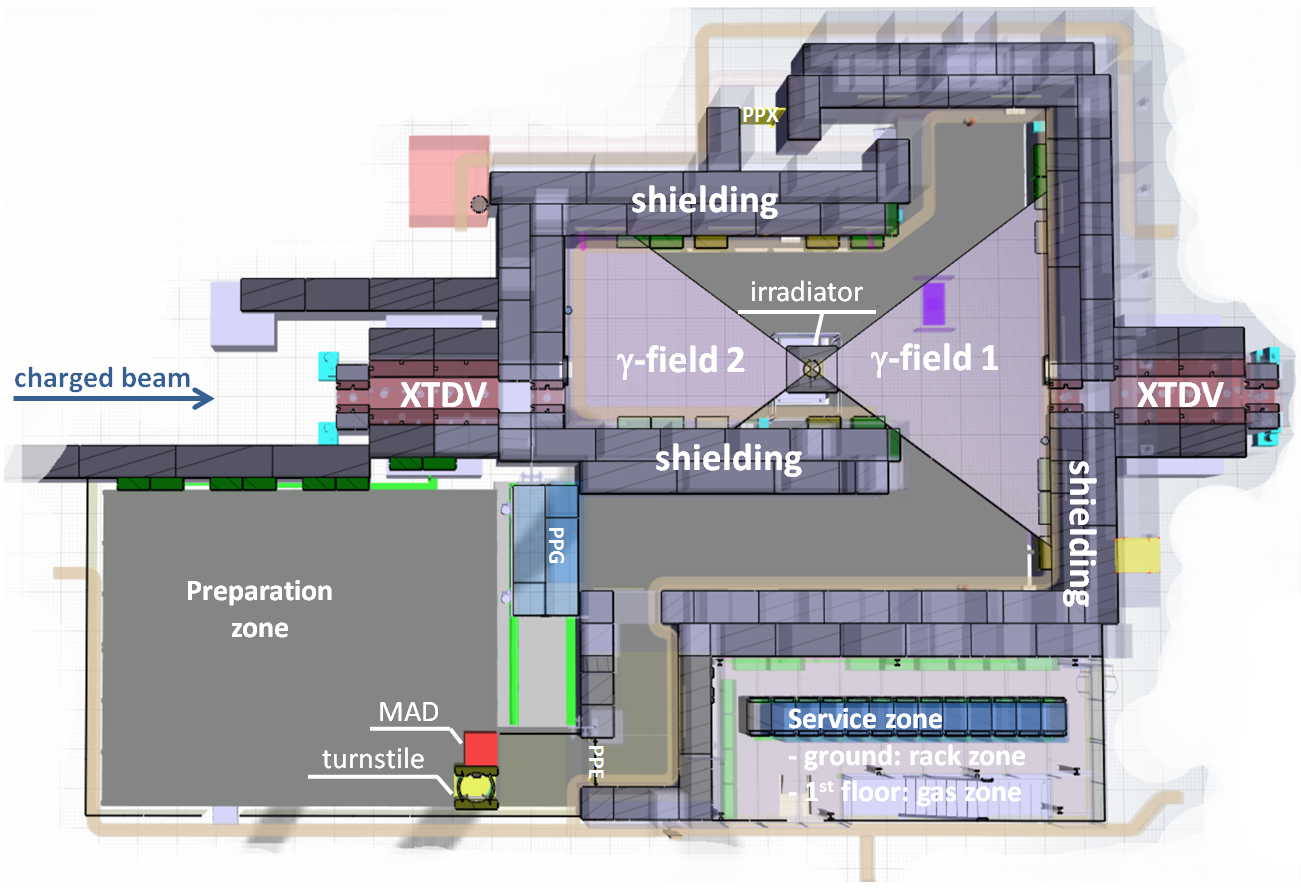
\includegraphics[scale=0.35]{images/GIF.png}
 \caption{An overview of the GIF++.}
\label{gif}
\end{figure}

\begin{figure}[htp]
\centering
\hspace{-0.5cm}
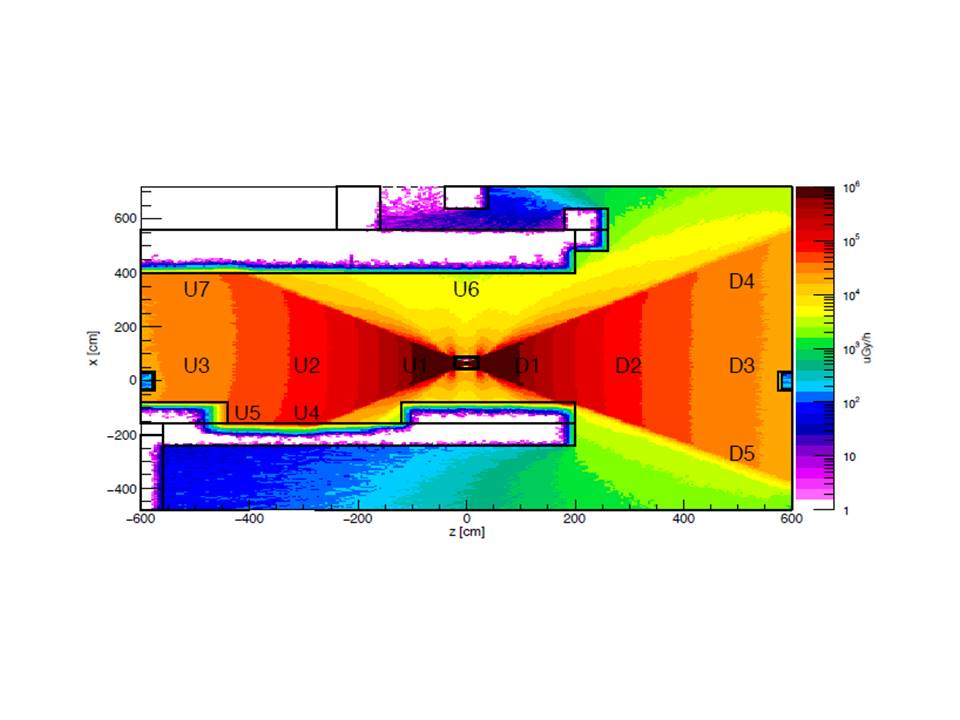
\includegraphics[scale=0.5,trim=60 130 60 130,clip]{images/simulation.jpg}
 \caption{Shows simulation of the source. The source lies at origin while `D' denotes the downstream region and `U' denotes the upstream region. The dose rate ranges from 10 to 10$^{6} \mu$Gy/h. }
\label{source}
\end{figure}

\section{WinCC-OA}Large experiments at CERN use WinCC-OA as a tool to develop control systems. It has capabilities to describe a device in the form of a data point and its elements which can be used for reading and writing to corresponding device. The devices can be accessed via OPC (OLE (Object Linking and Embedding) for Process Control) server \cite{opc}. Parameters of interest can be stored in the data base and used for trending and offline analysis. WinCC-OA gives a User Interface (UI) facility and access to the system using Access Control System.

\section{The CMS RPC DCS project in GIF++}
The CMS RPC DCS at GIF++ has been developed by using WinCC-OA 3.11 tool, which is further extended with the standard Joint Control Project (JCOP) framework \cite{jcop}. The JCOP framework provides extra functionalities such as the Finite State Machine (FSM), the Graphical User Interface (GUI), the alarm handler and the ORACLE data base interface \cite{g-polese}. The project controls the High Voltage and Low Voltage system through the OPC protocol. The environmental and gas sensors ( for pressure, temperature and humidity) are also readable via the OPC protocol. The source status and attenuator values are available centrally via the Data Interchange Protocol (DIP). The project has been designed as a distributed one to be able to communicate with other projects and to read valuable information. Communication has been established with the central GIF++ DCS, such that the information from the gas system, like flow rates are readable.\\
The Finite State machine (FSM) hierarchy of the project is based on the naming convention of the trolley, where the detectors are installed. Each trolley has six sections and each section accommodates one detector. Currently three CMS RPCs trolleys are installed in the GIF++. Trolley 1 (RPC Consolidation) is equipped with spare RPCs, trolley 2 with small glass RPCs and trolley 3 with prototypes of improved RPCs. Detail information of the trolleys are given here \cite{salvador}. 
A schematic overview of DCS project is shown in Fig:\ref{DCS_sys}. 

\begin{figure}[htp]
\centering
\hspace{-0.5cm}
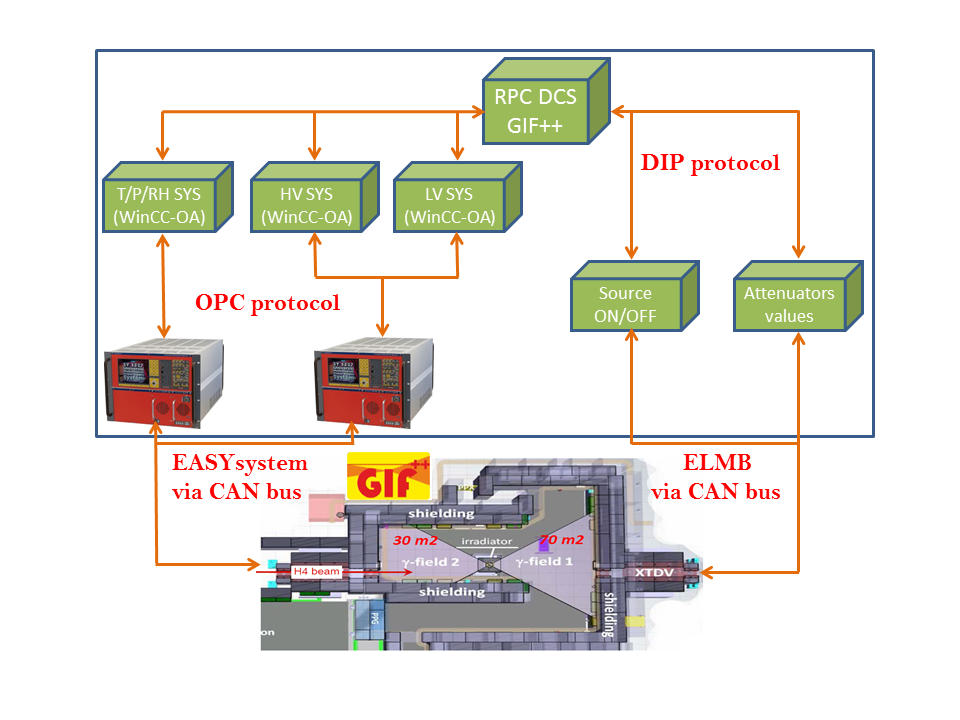
\includegraphics[scale=0.5,trim=60 30 60 30,clip]{images/DCS_sys.png}\\
 \caption{DCS project overview.}
\label{DCS_sys}
\end{figure}

 
\subsection{High and Low Voltage System}
The High and Low Voltage system is controlled and monitored by the CAEN OPC server. Each gap of a chamber is independently connected to a single HV channel which improves the granularity of chambers. The RPC front-end electronics requires digital and analog power supplies \cite{feb}. Each LV line is shared between two front-end-boards (FEBs) for digital as well as for analog. The LV boards are installed in the CAEN main frame and controlled by DCS. 
 
\subsection{Environmental and Gas Parameters}
The performance of RPCs strongly depends on the temperature and pressure of the environment \cite{env-rpc}. Therefore, it is important to measure the environmental parameters (temperature, pressure and humidity) at different locations. The applied voltage is corrected for the environmental temperature and pressure using the
following formula.
\begin{equation*}\label{veff}
V_{eff} = V_{0} ( 0.2 + 0.8 (\frac{P}{P_{0}} \times \frac{T_{0}}{273+T}))
\end{equation*}
where P and T are environmental pressure and temperature respectively while $P_{0} = 990$ and $T_{0} = 293$ are reference pressure and temperature respectively. Pressure is measured in mbars and temperature in K. The environmental and gas sensors (temperature, pressure and humidity) are readable through ADC (analog-to-digital converter) board which is installed in EASY crate. The JCOP framework gives the oppertunity to convert oline the ADC values into ordinary values of temperature (C$^o$), pressure (mb) and humidity (\%). The trending feature provides a comparison among different sensors located at different positions.

\subsection{High Voltage Scan and Stability Test}
As the project is designed for R\&D of detectors, most of the time some high voltage scanning or stability tests are running. For high voltage scanning a separate branch is made in the FSM tree where a user operates each detector independently. The stability test runs for a long time and it is necessary to restart the application if it stops. Based on the requirements, a dedicated manager is running to apply the stability script and restart it automatically.    
\subsection{FSM and GUI} 
The JCOP framework provides Finite State Machine (FSM) toolkits in WinCC-OA based on State Machine Interface (SMI++). It offers an easy, robust and safe way to control the full detector through the definition of a finite number of states, transitions and actions (ON, OFF, STANDBY, Ramping Up, Ramping Down). All the DCS hierarchy nodes are implemented through the FSM mechanism.\\
WinCC-OA provides Graphic User Interface (GUI) panel- an intuitive tool to control and monitor the detector, easy to use by non-experts and safe operation of the detector. It gives the opportunity to combine text, graphical objects and synoptic diagrams. GUI panels can be used to see the online behavior of the detector in the form of plots, tables and histograms. 

\begin{figure}[H]
\centering
\hspace{-0.50cm}
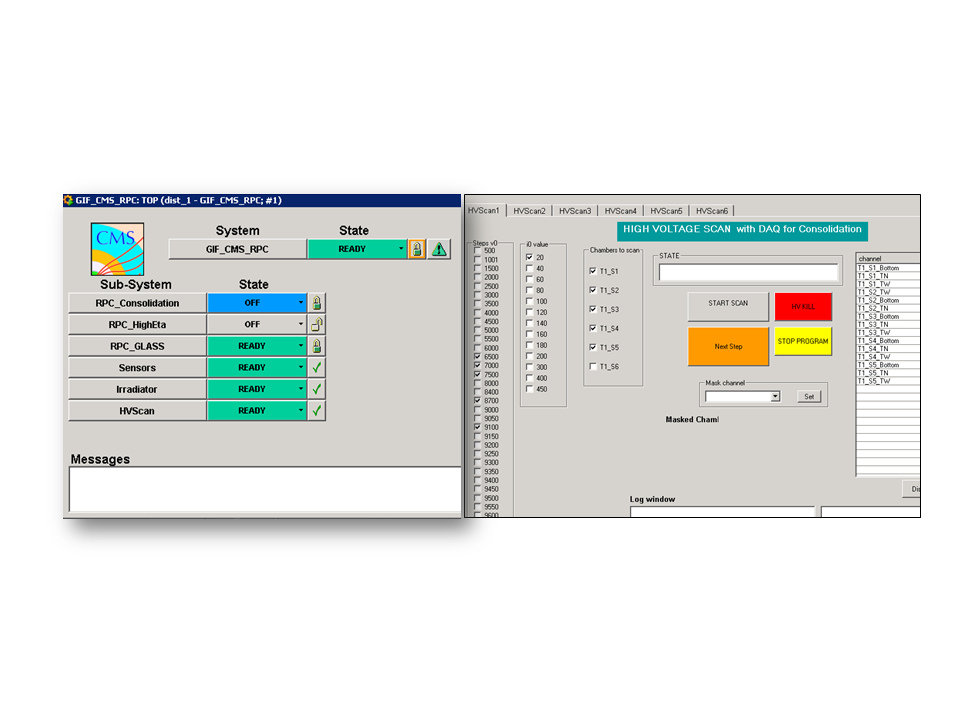
\includegraphics[scale=0.66,trim=30 150 30 140,clip]{images/GUI.png}\\
 \caption{FSM main tree and HV Scan panel using GUI.}
\label{gui}
\end{figure}

\section{Data Base}
To study the behavior of the detector over time and to make offline data analysis, it is necessary to store all the important parameters in a data base. WinCC-OA has its internal ORACLE data base which is used in this project. The stored data is extracting within the domain of the project and using for trending and offline analysis.  

\section{Conclusion} 
A DCS project for CMS RPCs is successfully tested and implemented in the CERN GIF++. Since June, 2015 the project is running in a stable state, operating the detector and archiving the data. The hardware is integrated in the project, fully controlling high voltage scanning and stability tests. The environmental and gas sensors are included and used for T/P corrections. Gas flowmeters are reading through central DCS at GIF++ and the data are using to study the behavior of different gases. All useful parameters are archiving in the internal data base for trending and offline analysis. As the project is designed for detector R\&D study, any new hardware can be included in easy and safe mode.  

\acknowledgments
Many thanks to Marino Romano for his technical support to develop the project.   

% We suggest to always provide author, title and journal data:
% in short all the informations that clearly identify a document.

\begin{thebibliography}{99}
\bibitem{gif} M. R. Jakel et. al., \emph{CERN GIF++: A new irradiation facility to test large-area particle detectors for the high-luminosity LHC program.}
\texttt{PoS(TIPP2014)102.} 
\bibitem{atlas-gif} B. Alvarez Gonzalez et. al., \emph{Ageing Studies on the First Resistive-MicroMeGaS Quadruplet at GIF++, }\texttt{EDP Sciences, 2015.}
\bibitem{wincc-oa} \href{https://wikis.web.cern.ch/wikis/display/EN/WinCC-OA+Service}{\texttt{wikis.web.cern.ch/wikis/display/EN/WinCC-OA+Service}}.
\bibitem{opc}OPC Servers: An introduction,
\href{http://www.cyberlogic.com/cyberlogic/docs/tutorials/OPC\_Server\_Tutorial.pdf}{\texttt{http://www.cyberlogic.com/cyberlogic/docs/tutorials/OPC\_Server\_Tutorial.pdf}}
\bibitem{jcop}The CERN Engineering Department, \emph{JCOP Framework Project},
\href{https://wikis.web.cern.ch/wikis/display/EN/JCOP+Framework}{\texttt{https://wikis.web.cern.ch/wikis/display/EN/JCOP+Framework}}
\bibitem{g-polese}G. Polese et. al., \emph{The Detector Control Systems for the CMS Resistive Plate Chamber, }\texttt{J. Phys. Conf. Ser. 219 022019.}
\href{http://iopscience.iop.org/article/10.1088/1742-6596/219/2/022019/pdf}{\texttt{doi:10.1088/1742-6596/219/2/022019}}
\bibitem{salvador}Salvador Carrillo Moreno et. al., \emph{CMS RPC preliminary results for aging studies at new CERN GIF++ facility}, proceedings from the XIII RPC worksop and related detectors.
\bibitem{feb}The CMS Collaboration, \emph{The Muon Project Technical Design Report}, CERN/LHC 97-32, CMS TDR 3, 15 December 1997.
\bibitem{env-rpc}Q Zhang et al., \emph{Environmental Dependence on the Performance of the Resistive Plate Chambers, }\texttt{2010 JINST 5 P02007.}
\href{http://iopscience.iop.org/article/10.1088/1748-0221/5/02/P02007/pdf}{\texttt{doi:10.1088/1748-0221/5/02/P02007}}

\end{thebibliography}
\end{document}
